\chapter{Ice Reservoirs}

\cleanchapterquote{Glaciers are the secret of life in these otherwise lifeless deserts. But now, they are
	melting away at an alarming rate.}{Sonam Wangchuk}{(Ramon Magsaysay awardee,\\ Inventor of ice stupas)}


\section{Introduction}

Mountains contribute disproportionally to global water resources compared with their geographical extent.
Because of their buffering capacity, for instance by supplying glacial melt water during the hot and dry season,
they provide a relatively constant water supply to downstream areas. Worldwide, the vast majority of glaciers
are losing mass \citep{zempGlobalGlacierMass2019a}, snow melt dynamics are being perturbed
\citep{mukhopadhyayReevaluationSnowmeltGlacial2015, hammondGlobalSnowZone2018}, and precipitation and
evapotranspiration patterns are shifting, all leading to future vulnerability of mountain water availability
\citep{lutzConsistentIncreaseHigh2014}. There is high confidence that these changes are largely negatively
impacting agriculture across many different mountainous regions \citep{ipccCrossChapterPaperMountains2022}.

These issues are particularly pronounced in arid and semiarid regions, where it is estimated that between 50 \%
and 90 \% of freshwater resources originate from mountain catchments
\citep{mukhopadhyayReevaluationSnowmeltGlacial2015, messerliMountainsWorldVulnerable2004}. As a consequence,
mountain communities have developed some nature-based water storage solutions and farming practices, namely,
bofedales \citep{monge-salazarEcohydrologyEcosystemServices2022}, amunas
\citep{ochoa-tocachiPotentialContributionsPreInca2019}, rock glacier oasis \citep{pandeyRockGlacierOasis2022}
and \ac{AIRs} \citep{wangchukIceStupaCompetition2020} to cope with climate change induced water stress.

\citet{immerzeelImportanceVulnerabilityWorld2020} quantify the importance of these mountain regions by
classifying river basins as \ac{WTUs}. Globally there are 78 \ac{WTUs}, which are home to more than 250 million
people. Among these, the most important WTUs lie in Central Asia where communities are increasingly relying on
\ac{AIRs} for climate change adaptation (Fig. \ref{fig:WTUs_AIRs}). 

There is a long tradition of building \ac{AIRs} with records dating back to more than 50 years
\citep{nusserSociohydrologyArtificialGlaciers2019}. \ac{AIRs} capture water in the autumn and winter, allowing
it to freeze, and hold it until spring, when it melts and flows down to the fields
\citep{ipccChapterHighMountain2019, vinceGlacierMan2009, clouseLadakhArtificialGlaciers2017,
nusserSociohydrologyArtificialGlaciers2019}. In this way, they retain a previously unused portion of the annual
flow and facilitate its use supplementing the decreased flow during the following spring (Fig.
\ref{fig:irrigation_cycles}). Over the past decade, several \ac{AIRs} have been built to supplement the
irrigation water supply of mountain villages in India \citep{wangchukIceStupaCompetition2020,
palmerStoringFrozenWater2022, aggarwalAdaptationClimateChange2021}, Pakistan
\citep{awazproductionIceStupaArtificial2022}, Kyrgyzstan \citep{bbcnewsBrightArtificialGlacier2020}, Nepal, and
Chile \citep{reutersConservationistsChileAim2021}. In total, more than 500 farmers have constructed AIRs across
30 villages in the Alps, Andes and Hindu Kush Himalayas (Fig. \ref{fig:WTUs_AIRs}).

\begin{figure}[htb]
	\centering
	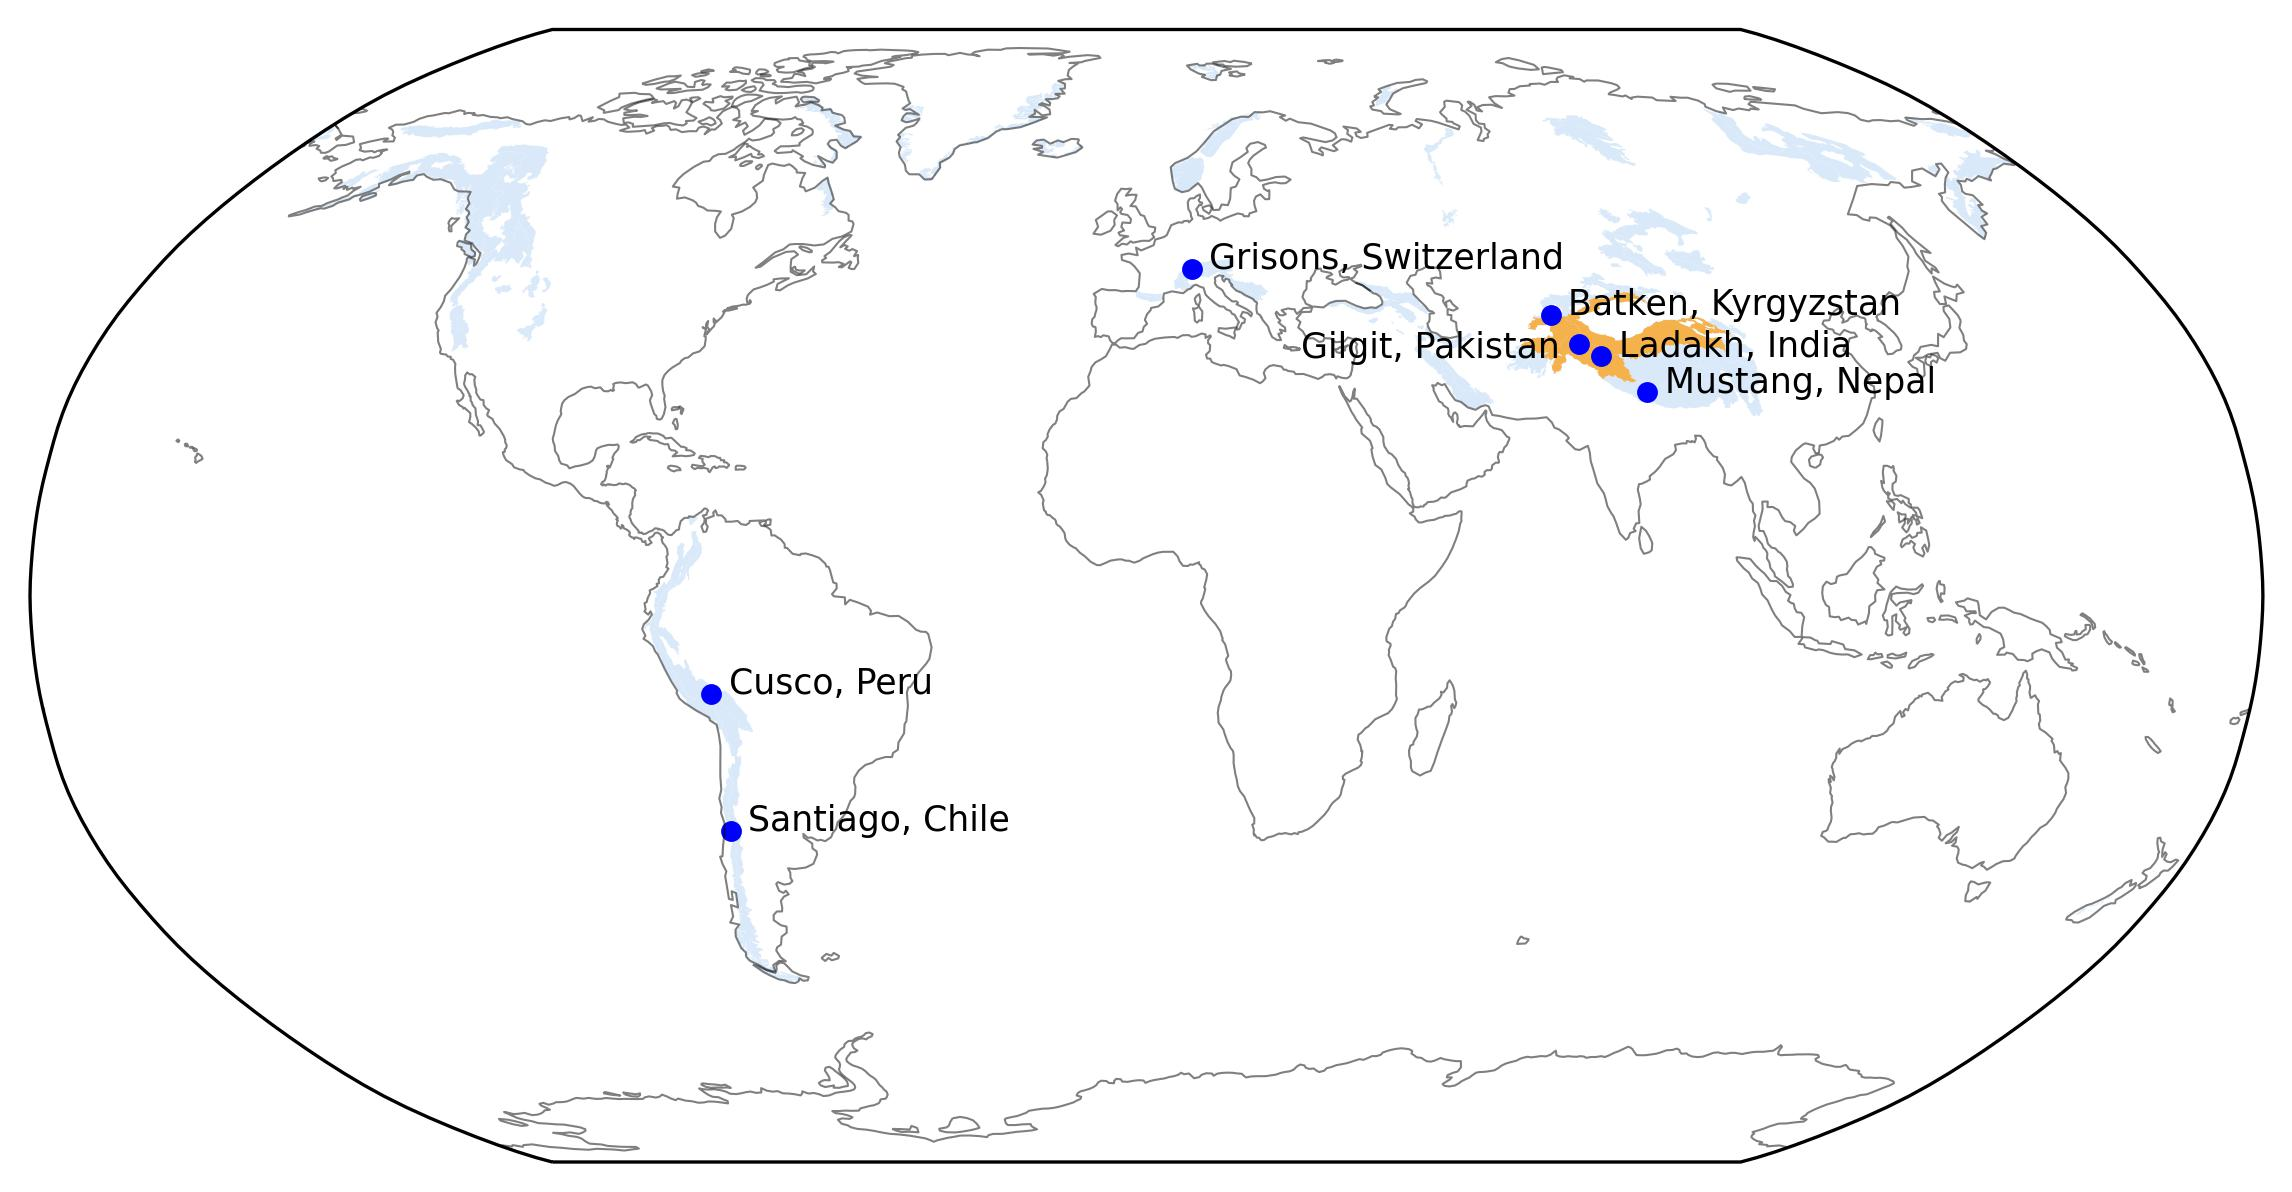
\includegraphics[width=\textwidth]{figs/WTUs_AIRs.jpg}

	\caption{ Global distribution of water tower units (light blue) based on
		\citet{immerzeelImportanceVulnerabilityWorld2020}. The most important \ac{WTUs} (orange) are also where most of
		the AIR construction sites  are located (dark blue). }

	\label{fig:WTUs_AIRs}
\end{figure}

\begin{figure}[htb] \centering 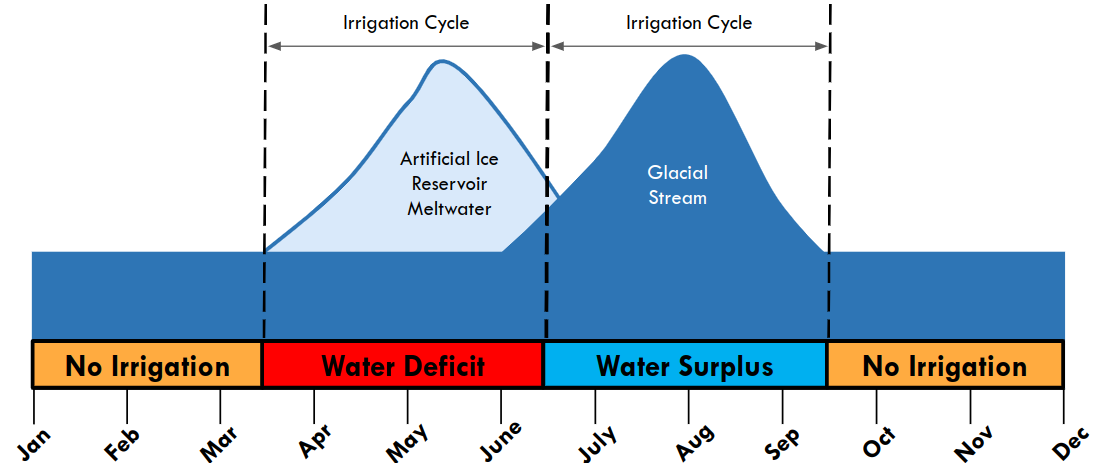
\includegraphics[width=\textwidth]{figs/irrigation_cycles.png}
	\caption{Seasonal variation in the availability of irrigation water in Ladakh, India. The graph highlights the
		crucial role of \ac{AIRs} in bridging the gap in water availability. Adapted from
		\citet{nusserLocalKnowledgeGlobal2016}.} \label{fig:irrigation_cycles} \end{figure}


Despite this widespread adoption, only a few publications examine the role of \ac{AIRs} in the water resource
management of these regions. Notably, none of these prior reports have investigated \ac{AIRs} outside Ladakh.
Moreover, the available estimates of water storage capacity of \ac{AIRs} in Ladakh vary widely
\citep{norphelSnowWaterHarvesting2015, baglaArtificialGlaciersHelp1998}.

Quantifying the water storage capacity of \ac{AIRs} is not straightforward since the processes by which
\ac{AIRs} are formed are complex. These processes are controlled by local topography, meteorology and the
construction strategies used. Modelling approaches to quantifying these processes exist on glacier surfaces but
they are not readily applicable for \ac{AIRs} due to their limited size, and comparatively more variable surface
area. Therefore, conventional modelling approaches used in glaciology need to be adapted in order to capture the
spatio-temporal scale of AIR surface processes. Furthermore, these modelling approaches need to be validated and
calibrated with comprehensive data from field measurements.

A spirit of improvisation guides the construction of \ac{AIRs} \citep{clouseLadakhArtificialGlaciers2017}.
Depending on the local topography and on how water is supplied, \ac{AIRs} can form as flat sheets or vertical
cones and are, therefore, referred as ice terraces and ice stupas respectively (Fig. \ref{fig:AIRforms}). This
has resulted in \ac{AIRs} exhibiting significant volume variations despite experiencing similar
meteorological conditions. For example, in Ladakh, India, ice terraces have attained volumes up to 30 times
larger than ice stupas \citep{nusserSociohydrologyArtificialGlaciers2019}. However, the processes driving these
differences can only be understood if the complete design methodology behind each construction is available.

\begin{figure}[t]
	\centering
	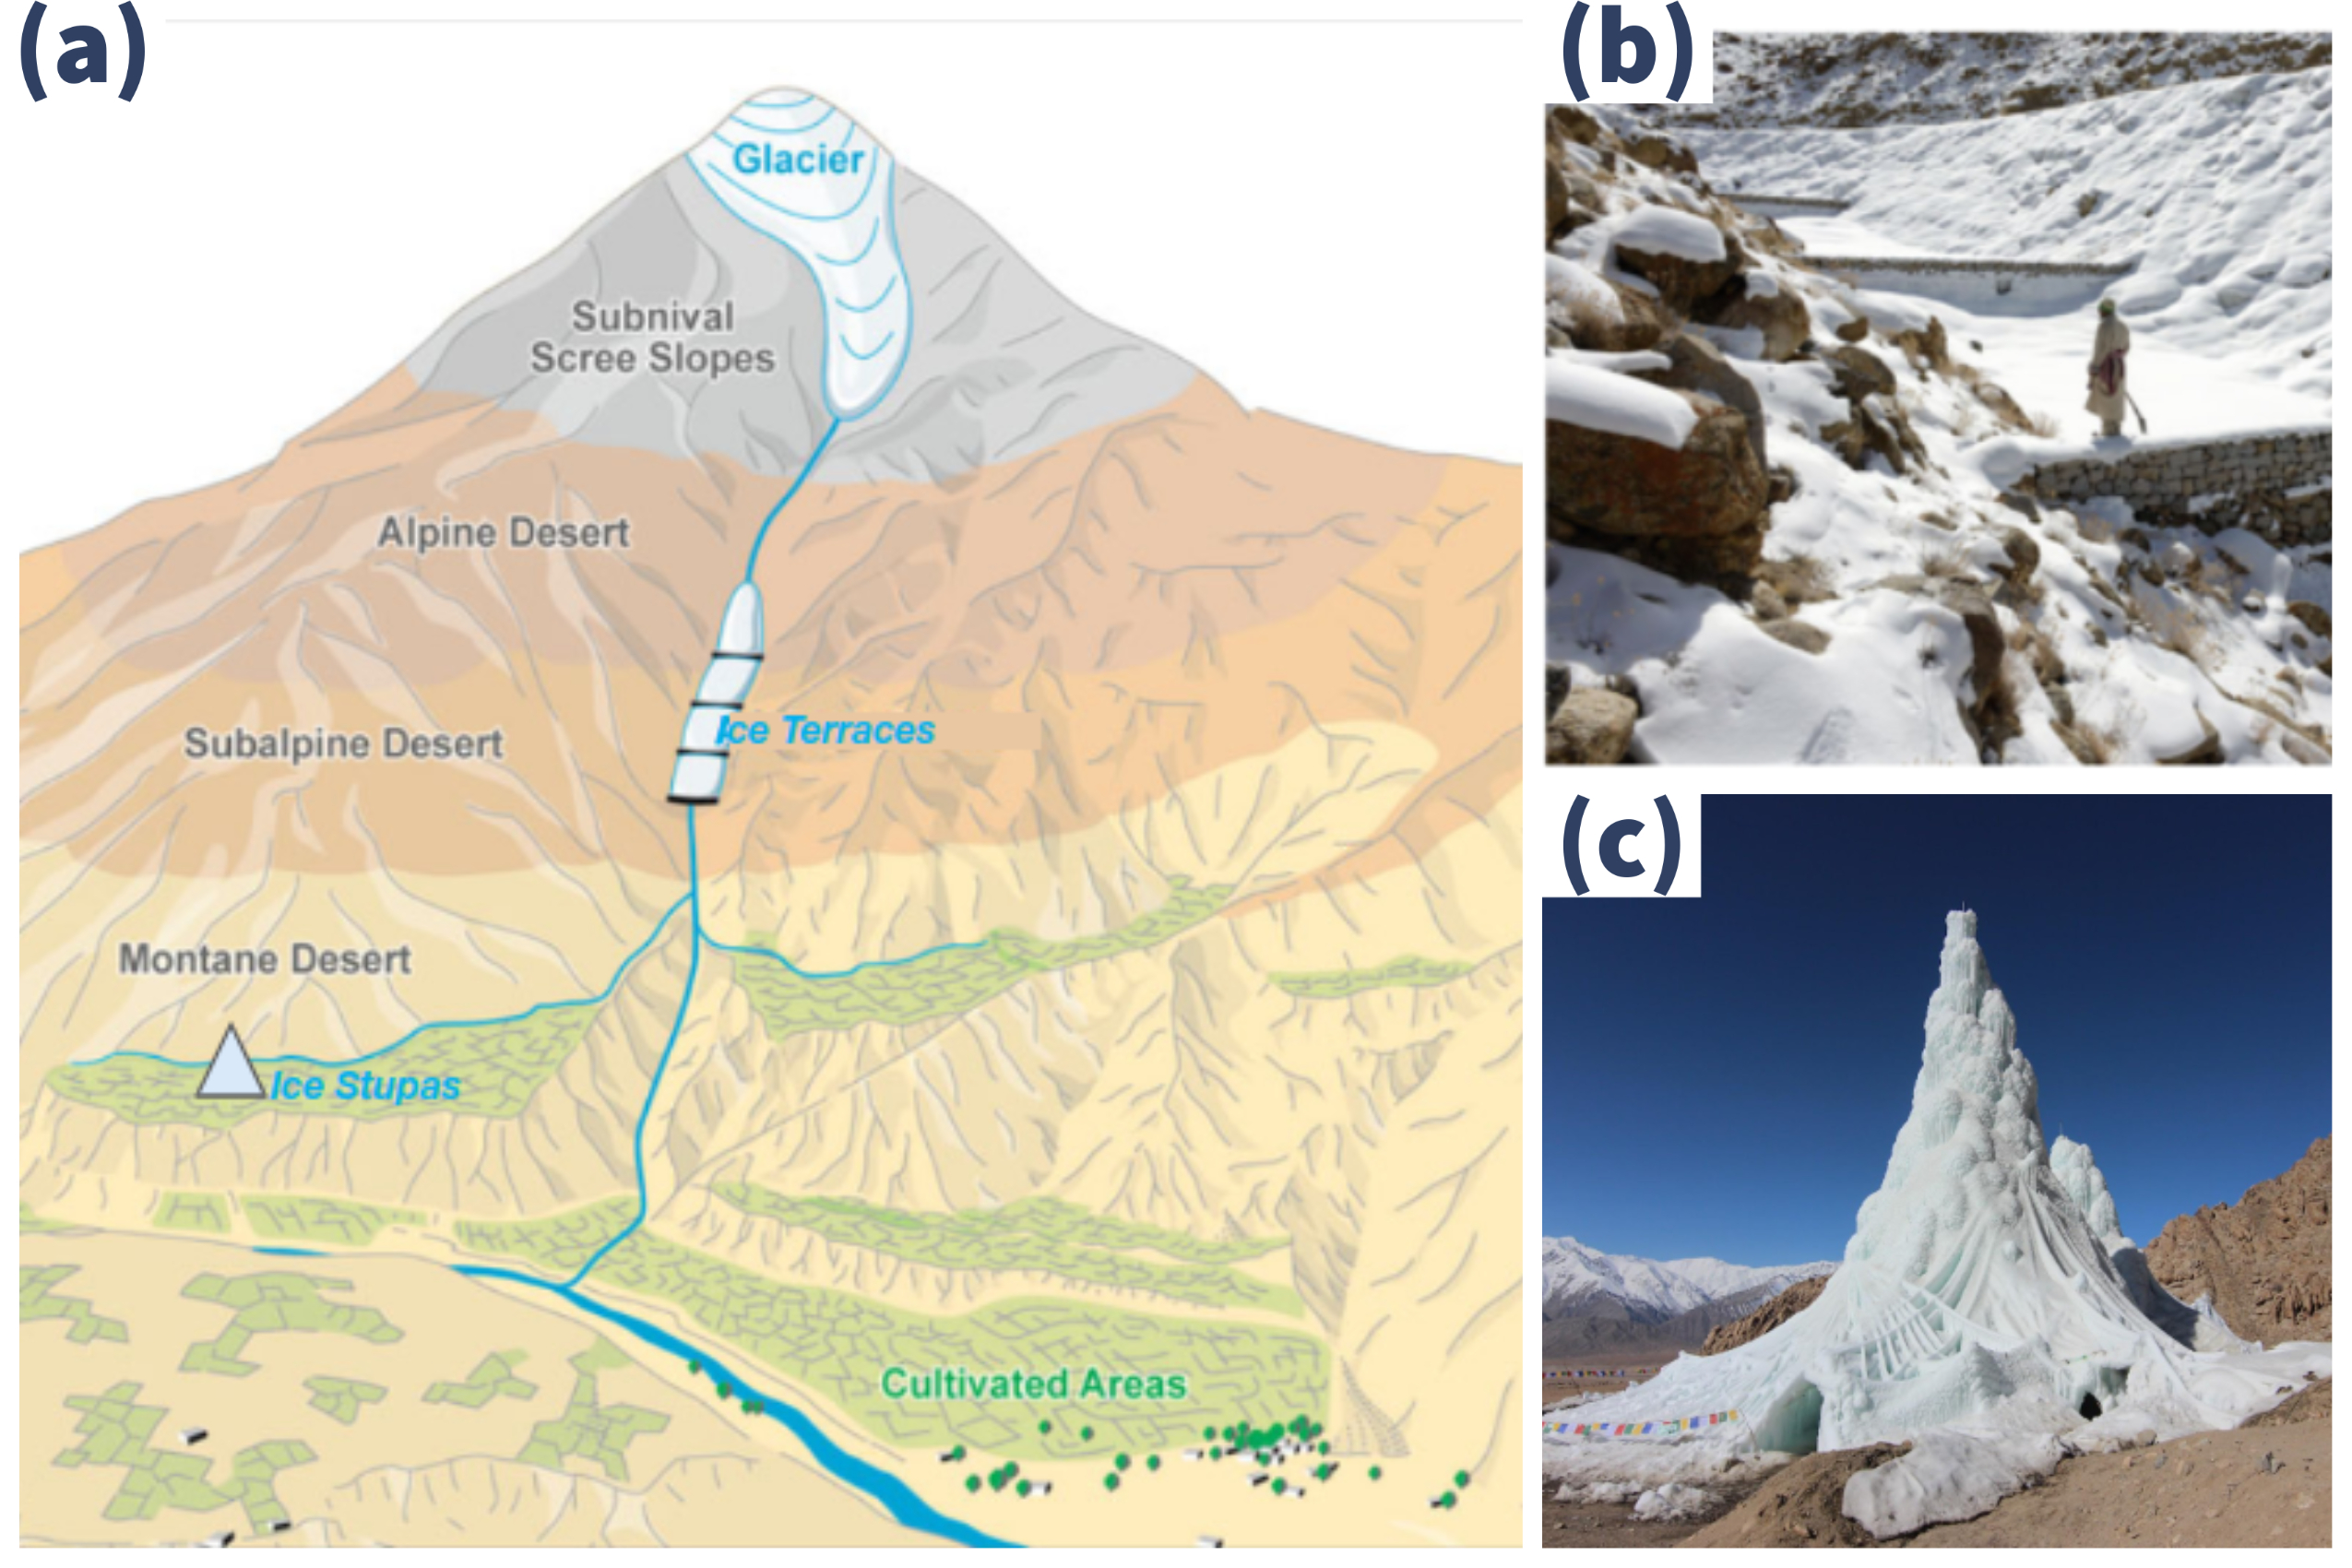
\includegraphics[width=\textwidth]{figs/AIR_forms.jpg}

	\caption{ (a) Schematic overview of the position of artificial ice reservoirs. These constructions are located at
		altitudes between the glaciers and the irrigation networks in the cultivated areas. (b) Ice terraces at 3900
		$m$ \ac{a.s.l.}, located above the village of Nang, Ladakh. The cascade is composed of a series of loose masonry walls
		ranging in height from 2 to 3 $m$, which help to freeze water for storage. (c) Ice stupas at 3600 m, located
		above the village of Phyang, Ladakh. They are made using fountain systems. Adapted from \citet{nusserLocalKnowledgeGlobal2016}. }

	\label{fig:AIRforms}
\end{figure}

This thesis aims to fulfill these requirements by providing a new set of AIR-specific volume and area
measurements via drone flights, along with meteorological data during the construction period. All these
datasets were generated through construction strategies that used fountain systems. These systems are quantified
via in-situ observations of the fountain characteristics and discharge rate measurements. First, one and two
dimensional models are formulated in order to calibrate and validate them with the procured AIR datasets. Then
these models are used as tools to propose a construction strategy that can produce \ac{AIRs} efficiently and
effortlessly. While this thesis reviews published research, we acknowledge that the farming communities building
these structures since the mid-1800s are the custodians of substantial additional knowledge.


\section{Nomenclature and Classification}

The term "artificial glacier" is more commonly used by local farmers to refer to \ac{AIRs}
\citep{norphelArtificialGlacierHigh2009}. However, many believe this terminology can be misleading
\citep{nusserSociohydrologyArtificialGlaciers2019}. By definition, all glaciers, including the smallest ones,
are bodies of sedimentary ice, which were built by progressive snow compaction and firnification and flow
downhill under the influence of gravity \citep{benndouglasGlaciersGlaciation2014}. Hence, because of their
genesis and composition, \ac{AIRs} differ from glaciers. Man-made ice structures typically have a lifetime in
the order of months and a size million times smaller than typical glaciers. We use the terminology \ac{AIRs} to
distinguish the man-made ice structures described in this thesis from the natural ones.

However, when classified in terms of size and survival duration, \ac{AIRs} exhibit similar characteristics to
very small glaciers. The glossary of glacier mass balance and related terms by
\citet{cogleyGlossaryGlacierMass2010} defines very small glaciers or glacierets as follows:

\begin{thesis_quotation}
	A very small glacier, typically less than 0.25 $km^2$ in extent, with no marked flow pattern
	visible at the surface. To qualify as a glacieret, an ice body must persist for at least two consecutive
	years. Glacierets can be of any shape, and usually occupy sheltered parts of the landscape. Windborne snow and
	avalanches can be dominant contributors to the accumulation of glacierets.
\end{thesis_quotation}

This rather broad definition of glacierets or very small glaciers may be best suited to describe AIRs, since
they have been measured with areas as high as 0.15 $km^2$ \citep{nusserSociohydrologyArtificialGlaciers2019} and
observed to last beyond a year.

As noted above, AIR's construction strategies are usually inspired by a spirit of improvisation which challenges
their classification. However, it has been found that construction strategies using fountain systems form
conical \ac{AIRs}, while those that don't, form flat sheets of ice. \ac{AIRs} using fountain systems are called
"ice stupas" and those without are called "ice terraces" as this terminology denotes the resulting shape of the
respective \ac{AIRs} appropriately.

\section{Research aim and outline}

The preceding sections reveal that many of the small scale surface processes that occur on \ac{AIRs} are complex
and not well understood at present, and their interplay remains uncertain. To be able to better predict their
water storage potential and improve their water storage efficiency in different climates with varying
construction methodologies, they are important to unravel. In this thesis, the main objective therefore is:

\begin{thesis_quotation}

  \textbf{To increase the understanding of volume dynamics of artificial ice reservoirs in order to
  integrate this tool in the water resource management plan of mountain catchments.}

\end{thesis_quotation}

Data on \ac{AIRs} are scarce, which is the reason for many of the unknowns and uncertainties around the dynamics
of these ice structures. This thesis therefore has a strong focus on implementation of measurement campaigns
using drones and \ac{AWS} to reach the main objective. The thesis touches on two different topics that
addresses the following specific research questions:

\begin{enumerate}

  \item \textit{What is the influence of construction location and fountain characteristics on ice stupa volume
    evolution?}

Three process-based models for ice stupas were designed to answer the first research question. Since in-situ
    measurements were required to run this model, we executed a measurement campaign in Switzerland and India
    during the past 4 winters (2018/19, 2019/20, 2020/21, 2021/22). These data sets provided the necessary
    input, calibration and validation data to model the evolution of ice stupas and study their sensitivity to
    meteorological conditions and fountain characteristics. Description of the study sites and overview of these
    models are presented in the \textit{Science} chapter. Results from their application are presented in the
    \textit{Habitat} chapter.

  \item \textit{How can ice stupa fountain systems be engineered to reduce their water losses and maintenance
    efforts?}

To answer this question, we developed a new construction strategy using an automation system. The automation
    hardware incorporated the models developed to regulate fountain discharge rate. The description of the
    automation system and the advantages over traditional construction strategies are presented in the
    \textit{Technology} chapter.

\end{enumerate}

Additional to the chapters above, the \textit{Religion} chapter illustrates the origin of ice harvesting solutions among
mythologies and religious practices. In the \textit{Heritage} chapter, I synthesize the research presented in this
thesis. I place it into a broader perspective, discuss its main findings, and provide recommendations and an
outlook for future research. The \textit{Literature} chapter lays out the peer-reviewed work supporting the conclusions of this
thesis.


